%----------------------------------------------------------------
%
%  File    :  optimization.tex
%
%  Authors :  David Lechner, FH Campus Wien, Austria
%
%  Created :  10 Oct 2019
%
%  Changed :  10 Oct 2019
%
%----------------------------------------------------------------


\chapter{Optimierung}
\label{chap:optimization}

Das Kapitel \textit{Optimierung} zeigt wie die Identifikation mit dem verwendeten Algorithmus verbessert werden kann. Es wird einerseits versucht, die Daten zu optimieren, wie zum Beispiel die Anzahl der \textit{Features} oder die Dauer der Trainingszeit. Andererseits wird auch die Methode durch geschickte Parametrisierung verbessert.

\section{Random Forest Parameter-Optimierung}
\label{sec:ml_optimization}

Die \textit{Random Forest} Implementierung von \textit{Scikit-Learn} bietet mehrere Parameter, welche die Trefferquote beeinflussen. Tabelle \ref{tab:rf_parameter} listet diese mit ihren Standardwerten und einer kurzen Beschreibung.

\begin{table*}[htbp]
  \centering
  \caption{\textit{Random Forest} Parameter \cite{sklearn_api}}
  \label{tab:rf_parameter}
  \begin{tabular}{|l|l|l|}
  \hline
  Parameter & Standardwert & Beschreibung\\
  \hline
  criterion & gini & \shortstack{Funktion zur Qualitätsmessung bei der Teilung.\\Mögliche Werte: \\gini: Gini-impurity \\entropy: Informationsgehalt} \\
  min\_samples\_split & 2 & \shortstack{Minimale Anzahl an Daten in einem Blatt,\\bevor es aufgeteilt wird} \\
  min\_samples\_leaf & 1 & Minimale Anzahl an Daten für ein Blatt \\
  max\_depth & None & Baumtiefe \\
  n\_estimators & 100 & Anzahl an \textit{Trees} im \textit{Forest}\\
  \hline
\end{tabular}
\end{table*}

Wie bereits im vorigen Abschnitt gezeigt, steuern die verwendeten Trainings- und Testdaten maßgeblich das \textit{Model}. Die Wahl der Parameter spielt dennoch eine Rolle. Um die Genauigkeit zu verbessern, können die Werte dahingehend angepasst werden. Damit es zu keinen Verfälschungen durch unterschiedliche Daten kommt, wurde jeder Optimierungsversuch sowohl mit denselben Trainings- als auch mit denselben Testdaten durchgeführt. Die Basis bildet daher ein 20-minütiges Datenset pro Fahrer, dessen Genauigkeit mit Standardparameter bei 91,28\% liegt. Zuerst ist jeder Parameter für sich verbessert und die Standardwerte der jeweils anderen herangezogen worden. Es wird nämlich angenommen, dass die Standardwerte bereits ein sehr gutes Ergebnis liefern. Jedoch auch, dass sich die Parameter gegenseitig beeinflussen, sodass die optimalsten Werte nur in Abhängigkeit der anderen bestimmt werden können.

\subsection{criterion}

Der erste Wert, den es zu verbessern gilt, ist \textit{criterion}. Er legt die Funktion fest, wie die Aufteilung bei einem Knoten durchgeführt wird und kann somit entweder \textit{gini} oder \textit{entropy} sein. Abbildung \ref{fig:rf_criterion} zeigt die Auswirkungen. Obwohl laut \cite{Rebala2019} \textit{entropy} für Kategorien besser geeignet ist, kann erkannt werden, dass die durchschnittliche Genauigkeit bei beiden etwa gleich ist. Jedoch fällt die Durchlaufzeit bei \textit{gini} (0.77 Sekunden zu 2.4) wesentlich kürzer aus. Für alle weiteren Optimierungen wurde daher auf Grund des besseren Zeitfaktors nur noch \textit{gini} verwendet.

\begin{figure}[htbp]
	\centering
	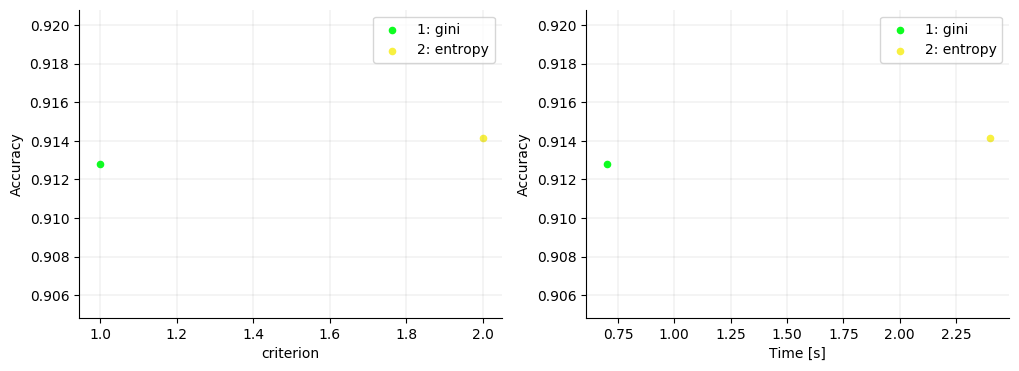
\includegraphics[width=\textwidth]{images/criterion_time.png}
	\caption{\textit{Random Forest} Parameteranalyse \textit{criterion}}
	\label{fig:rf_criterion}
\end{figure}

\subsection{min\_samples\_split}

Als zweites wird der Parameter \textit{min\_samples\_split} analysiert. Dieser bestimmt die mindest Anzahl an Datenpunkten in einem Knoten, welche für das Aufteilen notwendig sind. Auch hier wurden die Standardwerte für die anderen verwendet. Aus der Abbildung \ref{fig:rf_min_samples_split} geht hervor, dass der Parameter das Ergebnis um fast 1 Prozent beeinflusst (90.8 - 91.8\%), wobei die höchste Genauigkeit mit dem Wert \textit{3} erzielt wurde. Weiters ist zu erkennen, dass je höher der Parameter gewählt wird, desto geringer die Trefferquote ausfällt.

\begin{figure}
  \centering
  \begin{subfigure}[c]{0.45\textwidth}
    \centering
    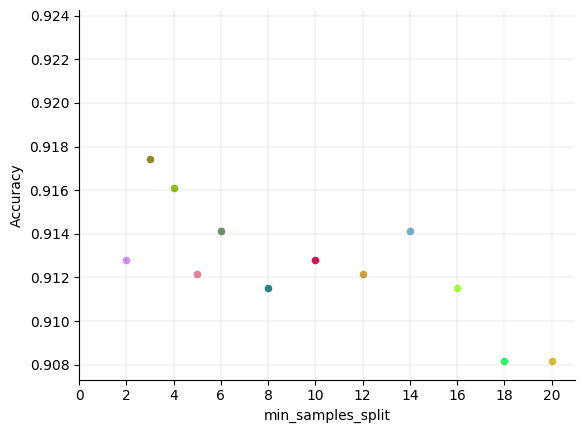
\includegraphics[width=\textwidth]{images/min_samples_split.png}
    \subcaption{\textit{min\_samples\_split}}
    \label{fig:rf_min_samples_split}
  \end{subfigure}
  \hfill
  \begin{subfigure}[c]{0.45\textwidth}
    \centering
    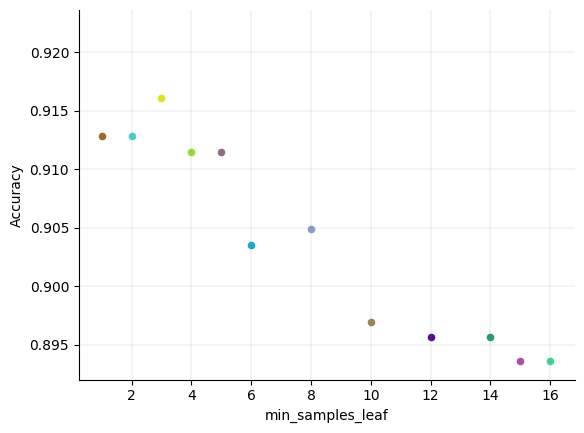
\includegraphics[width=\textwidth]{images/min_samples_leaf.png}
    \subcaption{\textit{min\_samples\_leaf}}
    \label{fig:rf_min_samples_leaf}
  \end{subfigure}
  \caption{\textit{Random Forest} Parameteranalyse}
\end{figure}

\subsection{min\_samples\_leaf}

Der nächste Parameter ist \textit{min\_samples\_leaf} und definiert die minimale Anzahl an Datenpunkten in den \textit{leaf nodes}. Wie die Abbildung \ref{fig:rf_min_samples_leaf} zeigt, nimmt auch hier die Genauigkeit mit ansteigenden Werten ab. Das Maximum liegt bei \textit{3} mit 91.16\%. Der Einfluss auf das ML-\textit{Model} ist etwas höher, da das schlechteste erzielte Ergebnis fast bei 89\% ist.

\subsection{max\_depth}

\textit{max\_depth} beschreibt die Baumtiefe. Ist der Wert auf \textit{undefined} (repräsentiert durch \textit{0} in der Grafik) gesetzt, wird ein Baum soweit expandiert, bis in einem Blatt \textit{min\_samples\_leaf} Datenpunkte erreicht werden. Das beste Resultat wird laut Grafik \ref{fig:rf_max_depth} bei einem Wert von \textit{15} erzielt. Danach fällt es leicht ab und pendelt sich ein.

\begin{figure}[htbp]
	\centering
	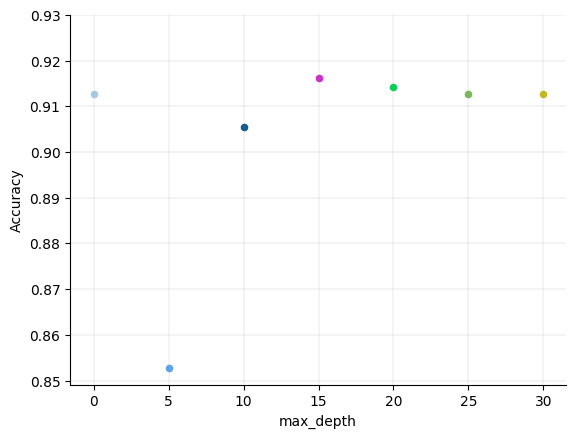
\includegraphics[width=0.5\textwidth]{images/max_depth.png}
	\caption{\textit{Random Forest} Parameteranalyse \textit{max\_depth}}
	\label{fig:rf_max_depth}
\end{figure}

\subsection{n\_estimators}

Die Anzahl der Bäume in einem \textit{Forest} werden durch den Parameter \textit{n\_estimators} spezifiziert. Laut Literatur \cite{Rebala2019}, steigt mit der Erhöhung der Anzahl auch die Genauigkeit des \textit{Models}. Die Abbildung \ref{fig:rf_n_estimators} bestätigt dies. Jedoch steigt auch die Trainings- beziehungsweise die Testzeit, was ebenfalls in der Grafik ersichtlich ist.

\begin{figure}[htbp]
	\centering
	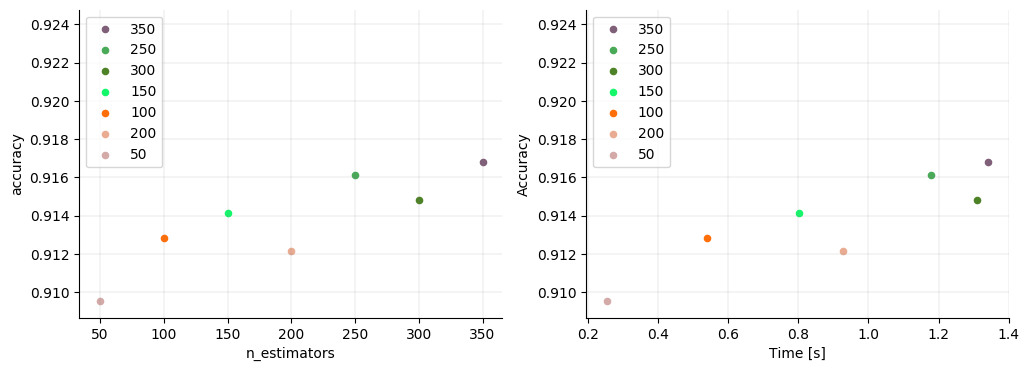
\includegraphics[width=\textwidth]{images/n_estimators.png}
	\caption{\textit{Random Forest} Parameteranalyse \textit{n\_estimators}}
	\label{fig:rf_n_estimators}
\end{figure}

\subsection{Verbesserte Parameter}

Die Tabelle \ref{tab:rf_best_std_parameter} zeigt unter anderem die Zusammenfassung der ersten Analyse. Wird nun das \textit{Model} mit diesen Werten auf die Daten angewendet, ergibt sich eine Genauigkeit von 91.41\%. Das heißt, es konnte lediglich eine Verbesserung um 0.13\% gegenüber den Standardwerten erreicht werden. Dies bestätigt die erste Annahme, dass die Defaultparameter bereits sehr gute Ergebnisse liefern. Weiters kann die Genauigkeit noch verbessert werden, in dem die beste Kombination aller Werte der Parameter gefunden wird. Hierfür müssen 16128 Tests mit dem \textit{Model} durchgeführt werden, was einen hohen Zeit- und Rechenaufwand bedeutet. Dabei ist eine größtmögliche Genauigkeit von 92.21\% herausgekommen, was einer Verbesserung von fast einem Prozentpunkt mit den Daten entspricht. Die Parameterwerte sind ebenfalls in der unten angeführten Tabelle ersichtlich. Gegenüber der ersten Analyse haben sich nicht mehr als zwei Parameter (\textit{min\_samples\_split} und \textit{n\_estimators}) verändert und das auch nur marginal. Für jede fortlaufenden Berechnungen wird diese Kombination verwendet.

\begin{table*}[htbp]
  \centering
  \caption{Verbesserte \textit{Random Forest} Parameter}
  \label{tab:rf_best_std_parameter}
  \begin{tabular}{|l|l|l|l|}
  \hline
  Parameter & Standardwert & Verbesserte Wert (mit Default) & Beste Kombination \\
  \hline
  criterion & gini & gini & gini \\
  min\_samples\_split & 2 & 3 & 3 \\
  min\_samples\_leaf & 1 & 3 & 1 \\
  max\_depth & None & 15 & None \\
  n\_estimators & 100 & 350 & 300 \\
  \hline
  \end{tabular}
\end{table*}

\section{Trainingszeit}

Die Trainingszeit eines ML-\textit{Models} wirkt sich unmittelbar auf die Genauigkeit der Ergebnisse aus. Je mehr Daten anfangs eingespeist werden, desto mehr kann das \textit{Model} lernen und ein genaueres Ergebnis bei neuen Daten liefern. Jedoch steigt auch die Wahrscheinlichkeit, dass die Anzahl an Datenpunkten höher wird, welche ungünstig für diese Anwendung sind. Die Genauigkeit sinkt wiederum dadurch. Laut \cite{Enev2016} und \cite{Ezzini2018} wird bei etwa zehn Minuten Trainingszeit eine Trefferquote von 90\% erzielt. Dies entspricht 300 Datenpunkte pro Fahrer. Die Autoren haben auch gezeigt, dass der allgemeine Fall - mehr Lernen für bessere Ergebnisse - hier nicht zwangsweise zutrifft. Ihre Modelle zeigen nach über 30 Minuten keine Verbesserungen mehr. Da aber auch nicht genau hervorgeht, mit welchen Daten sie zu diesen Erkenntnissen gekommen sind, wird dies versucht nachzustellen und zu validieren. Einerseits mit Daten, welche komplett zufällig aus dem ganzen Datenset mit allen Fahrern gewählt werden und andererseits mit Daten bei den ersten \textit{x} Minuten nach Fahrtbeginn. Dabei ist aber immer die Anzahl an Datenpunkten pro Fahrerin ident. Um eine genauere Aussagekraft der Analysen zu bekommen, wurden die Tests jeweils 50 mal mit unterschiedlichen Daten durchgeführt. Die Ergebnisse sind in den Abbildungen \ref{fig:train_duration_shuffle} und \ref{fig:train_duration_start} ersichtlich. Sie zeigen, dass zwischen zwölf und 18 Minuten an Trainingszeit mit Daten ab einem Fahrtbeginn die beste Trefferquote erzielt werden kann. Ab da an sinkt sie kontinuierlich. Dies deckt sich mit den Aussagen von \cite{Enev2016} und \cite{Ezzini2018}, wenngleich die Genauigkeit nicht konsequent erzielt werden konnte. Werden jedoch rein zufällige Daten für das Modell verwendet, ist erstens die durchschnittliche Genauigkeit (rote Linie) viel geringer, zweitens steigt sie mit der Anzahl der Daten und drittens gibt es weniger Ausreißer nach oben und nach unten je mehr Daten verwendet werden. Das Maximum liegt jedoch auch nur bei knapp über 76\% mit 40 Minuten an Trainingsdaten pro Fahrer. Es ist daher anzunehmen, dass die erwähnten Autoren nicht mit zufälligen Daten aus allen CAN-Signalen gearbeitet haben, sondern mit einem Subset.

\begin{figure}
  \centering
  \begin{subfigure}[c]{0.45\textwidth}
    \centering
    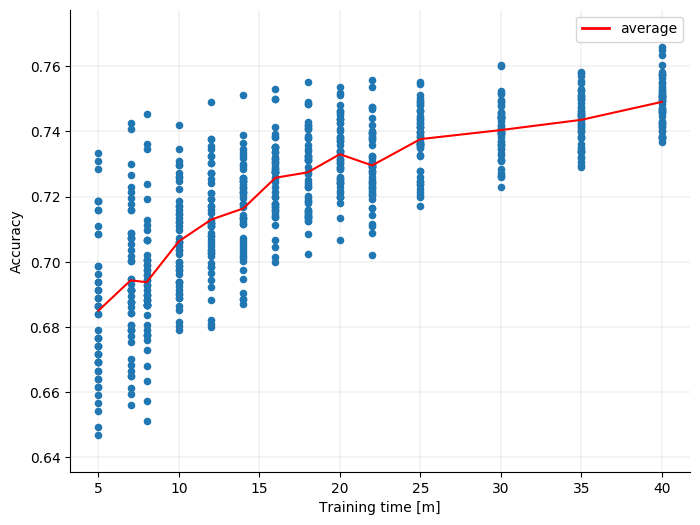
\includegraphics[width=\textwidth]{images/train_duration_shuffle.png}
    \subcaption{Analyse mit zufälligen Daten}
    \label{fig:train_duration_shuffle}
  \end{subfigure}
  \hfill
  \begin{subfigure}[c]{0.45\textwidth}
    \centering
    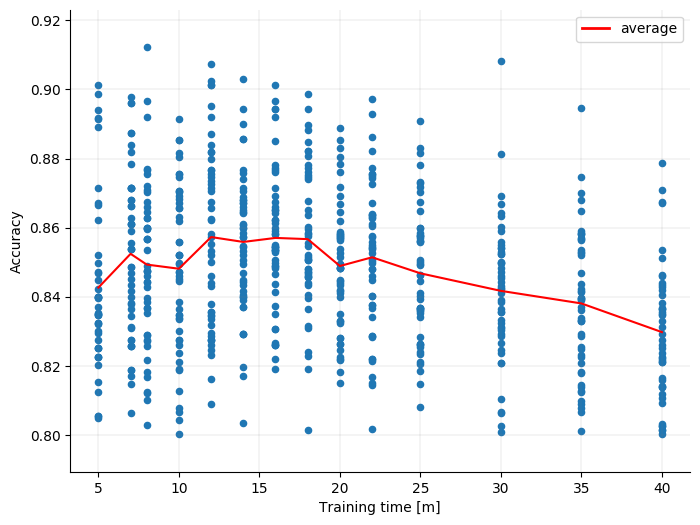
\includegraphics[width=\textwidth]{images/train_duration_start.png}
    \subcaption{Analyse mit Fahrtbeginn}
    \label{fig:train_duration_start}
  \end{subfigure}
  \caption{Analysen der Trainingszeit}
\end{figure}

\section{Feature Optimierung}
\label{sec:feature_optimization}

Eine weitere Möglichkeit das Modell zu optimieren ist, \textit{Features}, welche keine Auswirkung auf die Klassifizierung haben, zu entfernen. Dies spart Rechenleistung, -zeit und könnte unter Umständen auch das Endresultat verbessern. Hierfür gibt es mehrere Möglichkeiten.

\subsection{Feature Korrelationen}

Eine davon beschäftigt sich mit der Korrelation von \textit{Features} \cite{pittir8056}. Dabei wird analysiert, ob es zwischen Merkmalen einen Zusammenhang gibt. Es kann entweder der \textit{Pearson}- oder der \textit{Spearman}-Koeffizient herangezogen werden. Beide können Werte zwischen \textit{-1} und \textit{+1} annehmen. Ersterer kommt bei Daten zum Einsatz, welche sehr stark linear und kontinuierlich sind. Der zweite ist besser, wenn sich die \textit{Features} zusammen verändern, aber nicht unbedingt um den gleichen Faktor. Gibt es streng zusammenhängende Merkmale, können diese (bis auf eines) eliminiert werden. Dadurch reduzieren sich die zu verarbeitenden Daten und das spart Rechenaufwand. Bei den vorhandenen Daten ist anzunehmen, dass die verschiedenen \textit{Features} der einzelnen Signale - Minimal-, Maximal-, Durchschnittswert, Standardabweichung und Median - einen hohen Korrelationswert zueinander haben. Die Abbildung \ref{fig:feature_correlation} belegt dies mithilfe des \textit{Spearman}-Koeffizienten (\textit{+1}, dunkelblau). Daraus ist weiters zu erkennen, dass es einen offensichtlichen Zusammenhang zwischen dem Lenkradwinkel und den verschiedenen Kräften gibt, welche auf das Auto einwirken. Dies gilt ebenso für den Fahrpedalrohwert. Ansonsten können keine zusätzlichen Korrelationen ausgemacht werden.

\begin{figure}[htbp]
  \centering
  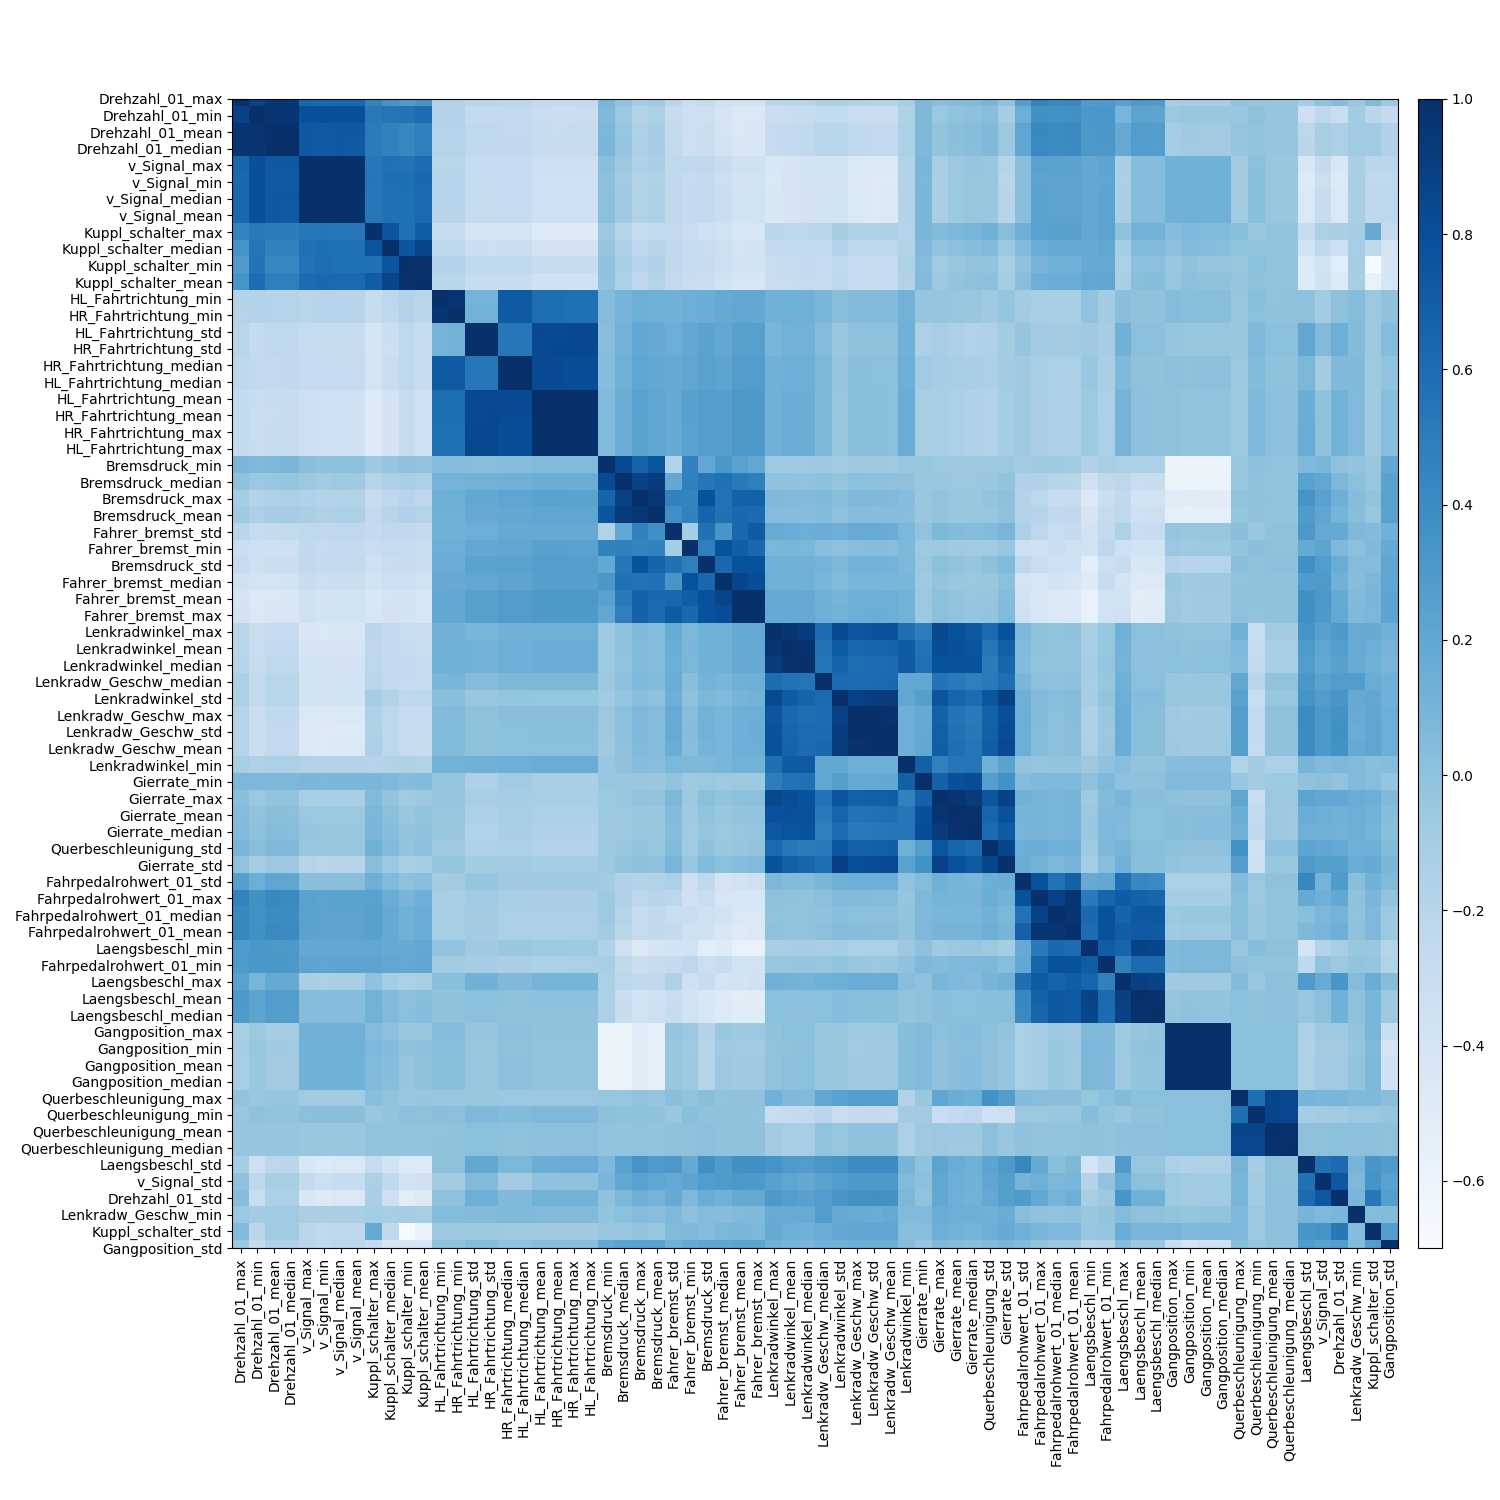
\includegraphics[width=0.9\textwidth]{images/feature_correlation.png}
  \caption{\textit{Feature} Korrelation}
  \label{fig:feature_correlation}
\end{figure}

\subsection{Feature Importance}
\label{sec:feature_importance}

Bevor jedoch einfach die stark korrelierenden \textit{Features} entfernt werden, kann noch eine weitere Analyse durchgeführt werden. Hierbei zeigt sich ein zusätzlicher Vorteil des Algorithmus \textit{Random Forest}. Wie bereits in den Grundlagen erklärt, wird nämlich mithilfe von \textit{Gini Impurity} das wahrscheinlich bestmögliche \textit{Feature} gefunden, um die Daten bei einem Knoten aufzuteilen. Dadurch kann bereits während der Erstellung der verschiedenen \textit{Decision Trees} festegellt werden, welchen Einfluss ein bestimmtes Datenattribut hat. Mit der Implementierung von \textit{Scikit-Learn} können genau diese Werte dargestellt werden. Aus der Abbildung \ref{fig:feature_importance} ist zu entnehmen, dass der Bremsdruck das stärkste Merkmal ist, um eine Fahrerin zu identifizieren. Dies deckt sich auch mit den Ergebnissen von Gahr et al., welche ausschließlich dieses Signal zur Identifizierung verwendet haben. Verwunderlich ist jedoch, dass die reine Gangposition die zweitgrößte Rolle einnimmt. Stellt man die Werte aller Fahrer über die gesamte Fahrzeit dar (siehe Abbildung \ref{fig:gear_position}), kann erkannt werden wieso. Für fünf Fahrer sind nämlich keine korrekten Werte vorhanden. Sie zeigen durchgehend den Gang 14. Dies kann mehrere Gründe haben. Entweder wurde das Aufzeichnungsgerät falsch konfiguriert, das falsche Signal in diesen Autos abgegriffen oder es war schlichtweg nicht vorhanden und 14 ist ein Standardwert. Auch bei den anderen Fahrzeugdaten dürfte ein Fehler unterlaufen sein, da zwischendurch der Gang 13 angezeigt wird. Aus diesem Grund ist für das ML-\textit{Model} die Gangposition so entscheidend. Soll ein neuer Datenpunkt klassifiziert werden, welcher den 14ten Gang enthält, kommen nur noch fünf Fahrer in Frage und dies nur Aufgrund des einen Signals. Es hat jedoch nichts mit dem Individuum hinter dem Lenkrad und dem Fahrverhalten zu tun. Infolge dessen werden dadurch die Ergebnisse des Modells verfälscht und das \textit{Feature} muss daher aus allen vorliegenden Daten entfernt werden. Da es wie erklärt die Trefferquote erhöht hat, geht damit auch ein Performance-Verlust einher. Im vorigen Abschnitt wurde gezeigt, dass mit den Daten eine maximale Genauigkeit von 92\% (durchschnittlich 86\%) erreicht werden konnte. Nach mehreren erneuten Durchläufen ohne der Gangposition konnte nun lediglich 80\% im Mittel und maximal 85\% erzielt werden. Das Modell hat sich demnach um mehr als 5\% verschlechtert, klassifiziert jedoch die Fahrer basierend auf korrekten Fahrzeugdaten.

\begin{figure}
  \centering
  \begin{subfigure}[c]{0.45\textwidth}
    \centering
    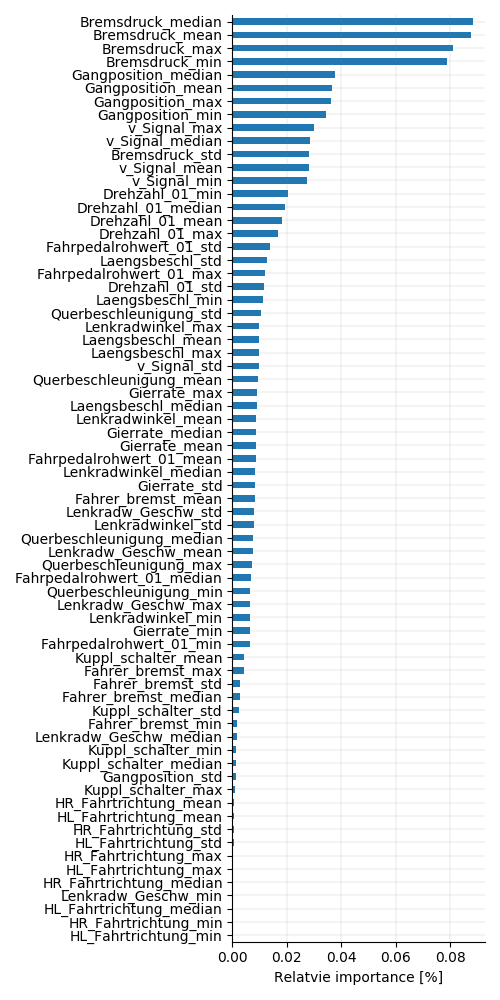
\includegraphics[width=\textwidth]{images/feature_importance.png}
    \subcaption{\textit{Scikit-Learn}s \textit{Feature Importance}}
    \label{fig:feature_importance}
  \end{subfigure}
  \hfill
  \begin{subfigure}[c]{0.45\textwidth}
    \centering
    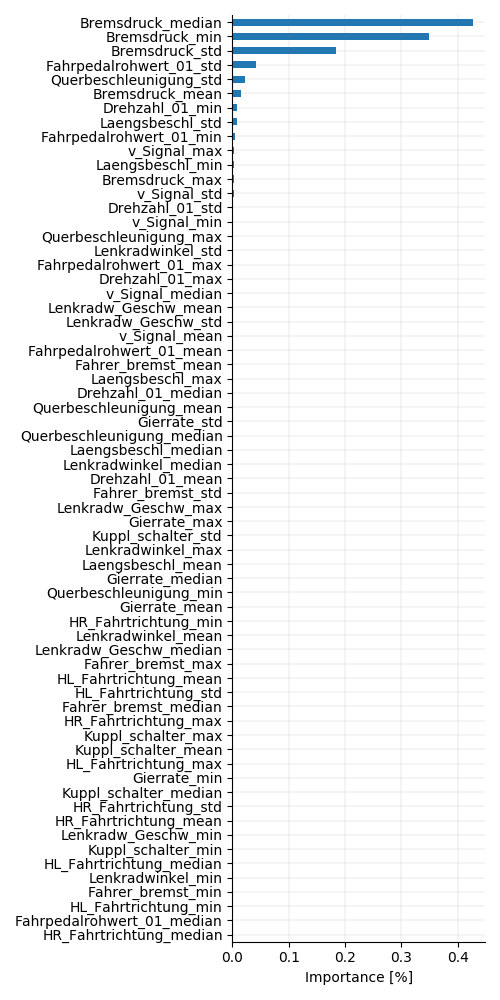
\includegraphics[width=\textwidth]{images/feature_perm_importance.png}
    \subcaption{\textit{Permutation Feature Importance}}
    \label{fig:feature_perm_importance}
  \end{subfigure}
  \caption{\textit{Feature Importance}}
\end{figure}

Des Weiteren zeigt die Grafik \ref{fig:feature_importance}, dass die Geschwindigkeit (\textit{v\_Signal}) und die Motordrehzahl ebenso einen großen Einfluss haben, obwohl eher das Gegenteil anzunehmen ist. Warum die Signale so weit oben angeführt werden hat vermutlich damit zu tun, dass die \textit{Feature}-Auswahl durch das \textit{Gini criterion} verzerrt ist. 2007 haben die Forscher Strobl et al. \cite{Strobl2007} folgendes herausgefunden: Ihre Versuche zeigen, dass \textit{Features} mit mehr potenziellen Aufteilungspunkten ein gutes Kriterium ergeben. Da diese Anzahl exponentiell mit der Anzahl der verschiedenen möglichen Werte steigt, werden solche Merkmale gegenüber welchen mit einer geringeren Varianz von \textit{Decision Trees} eher bevorzugt. Dafür haben sie ein zusätzliches Attribut mit reinen Zufallswerten in die Daten eingefügt. Bei der anschließenden \textit{Feature Importance}-Analyse haben sich diese Daten als besser gegenüber manch anderer echter Daten herausgestellt. Die Zufallswerte hatten dabei eine sehr große Varianz. Für die zwei genannten Signale trifft dies ebenso zu.

\begin{figure}[htbp]
  \centering
  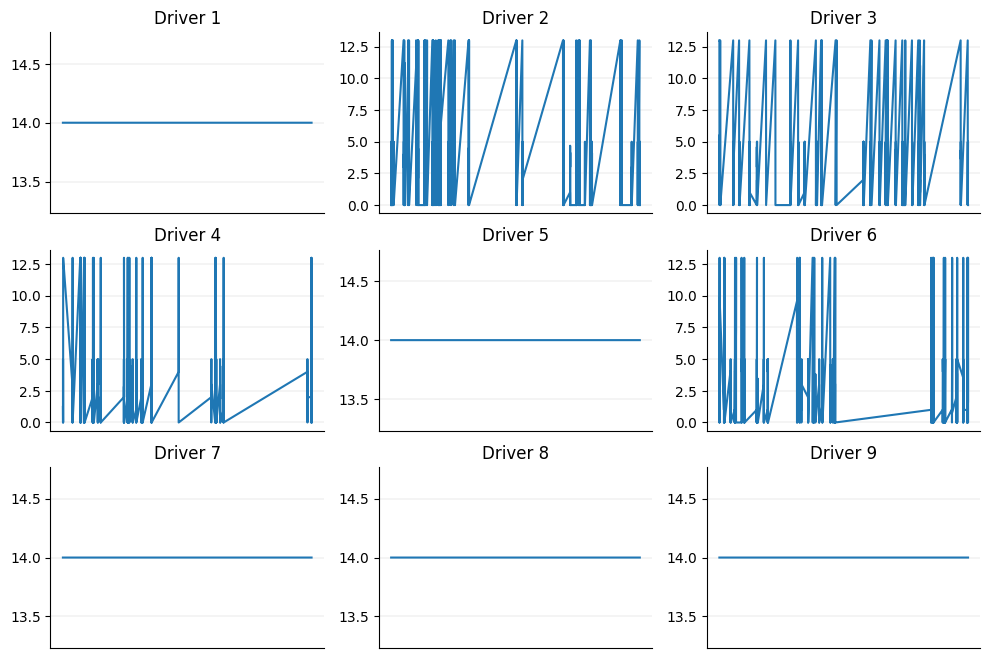
\includegraphics[width=0.7\textwidth]{images/gear_position.png}
  \caption{Gangposition}
  \label{fig:gear_position}
\end{figure}

\subsection{Permutation Importance}
Um diese Verzerrung durch das \textit{Gini criterion} zu umgehen, haben die oben genannten Forscher eine alternative Methode zur Messung der \textit{Feature Importance} vorgestellt \cite{Strobl2007}. Die Idee dahinter ist, herauszufinden, wie sich die Genauigkeit verändert, wenn ein bestimmtes \textit{Feature} nicht mehr existiert. So könnte zum Beispiel bei jedem erneuten Training des Modells eine Datenreihe weggelassen werden. Dies hat aber den Nachteil, dass es sehr Rechenaufwändig ist und nicht unbedingt wiederspiegelt, was in dem gesamten Datenset relevant ist. Einfach das bestimmte \textit{Feature} nur beim Testdurchlauf wegzulassen ist zwar billiger, funktioniert aber nicht, weil die trainierten Entscheidungsbäume alle Datenpunkte einer Reihe erwarten. Anstatt dessen können die echten Werte durch zufälliges Rauschen mit der gleichen Datenverteilung ersetzt werden. Das geht am leichtesten, wenn die Werte des gleichen \textit{Features} permutiert werden. Das Verfahren heißt daher \textit{Permutation Importance} und besteht aus folgenden drei Schritten, wobei Schritt zwei und drei sukzessive wiederholt werden:

\begin{description}
	\item[Schritt 1] Berechne die Genauigkeit des Modells mit allen \textit{Features}.
	\item[Schritt 2] Wähle ein \textit{Feature} aus, permutiere die Werte und berechne die Genauigkeit des Modells erneut.
	\item[Schritt 3] Die Differenz zwischen dem Wert aus Schritt 1 und Schritt 2 ergibt die Wichtigkeit des \textit{Features}.
\end{description}

Mittlerweile ist es als Funktion auch schon in dem \textit{Scikit-Learn} Modul zu finden und kann auf die Daten angewendet werden. Abbildung \ref{fig:feature_perm_importance} zeigt die Ergebnisse daraus. Hier ist zu erkennen, dass der Bremsdruck neuerlich das stärkste Kriterium ist. Das zweit bestbewertete Signal ist der Fahrpedalrohwert. Weiters bestätigt diese Messung die Annahme, dass es bei der ersten Methode eine Verfälschung gegeben hat, da die Geschwindigkeit und die Motordrehzahl weiter unten angeführt werden. Generell haben die meisten Signale eine geringere Auswirkung auf die Genauigkeit des Modells als anfangs gedacht. So sind beispielsweise der Lenkradwinkel, Lenkradbeschleunigung und die Kupplung sehr weit unten in der Tabelle. Das bedeutet aber nicht, dass diese Informationen gänzlich unwichtig für die Klassifizierung sind. Es heißt nur, dass sie für sich alleinstehend keine großen Auswirkungen haben, in Kombination hingegen vielleicht schon.

\subsection{Feature Selection}
\label{sec:feature_selection}

In den letzten zwei Abschnitten wurde die Korrelation zwischen den \textit{Features} gezeigt. Wenn die Eliminierung nach dieser Analyse geht, müssten nahezu $\frac{4}{5}$ der Merkmale wegfallen. Für die korrekte Auswahl kann die \textit{Feature Importance} von \textit{Scikit-Learn} herangezogen werden. Dabei wurden jedoch zwei Widersprüche festgestellt, zum einen die falschen Werte der Gangposition und zum anderen die Verfälschung durch das \textit{Gini criterion}. Mithilfe der Methode \textit{Permutation Importance} konnte dies bereinigt werden und einen möglichst unbeeinflussten Eindruck über die Wichtigkeit der \textit{Features} bekommen. Mit diesen Ergebnissen kann die sogenannte \textit{Feature Selection} durchgeführt werden, bei der die optimale Anzahl an Merkmalen in dem ML-\textit{Model} bestimmt wird. Zu diesem Zweck kann der Algorithmus \textit{Recursive Feature Elimination} (RFE) \cite{Guyon2002} verwendet werden. Als erster Schritt wird das Modell mit allen \textit{Features} trainiert und die Genauigkeit bestimmt. Danach kommt die Methode \textit{Permutation Importance} zum Einsatz, um die Wichtigkeit der Merkmale zu bestimmen. Anhand der resultierenden Reihung wird nach und nach das \textit{Feature} mit der geringsten Auswirkung eliminiert, bis nur noch eines (in diesem Fall \textit{Bremsdruck\_median}) über bleibt. Bei jedem Durchlauf erfolgt das erneute Antrainieren mit dem Subset der Merkmale und die Bestimmung der Genauigkeit. Der gesamte Vorgang wurde mit 100 verschiedenen Trainings- bzw. Testdaten durchgeführt. Werden die Resultate in einer Grafik visualisiert (siehe Abbildung \ref{fig:feature_selection}), kann erkannt werden, wie viele \textit{Features} für eine gewisse Trefferquote benötigt werden. So gibt es zwischen den ersten zehn Merkmale eine deutliche Steigerung und ab dem elften flacht sie ab. Ein sehr guter Wert kann mit 21 der verfügbaren 65 \textit{Features} erzielt werden.

\begin{figure}[htbp]
  \centering
  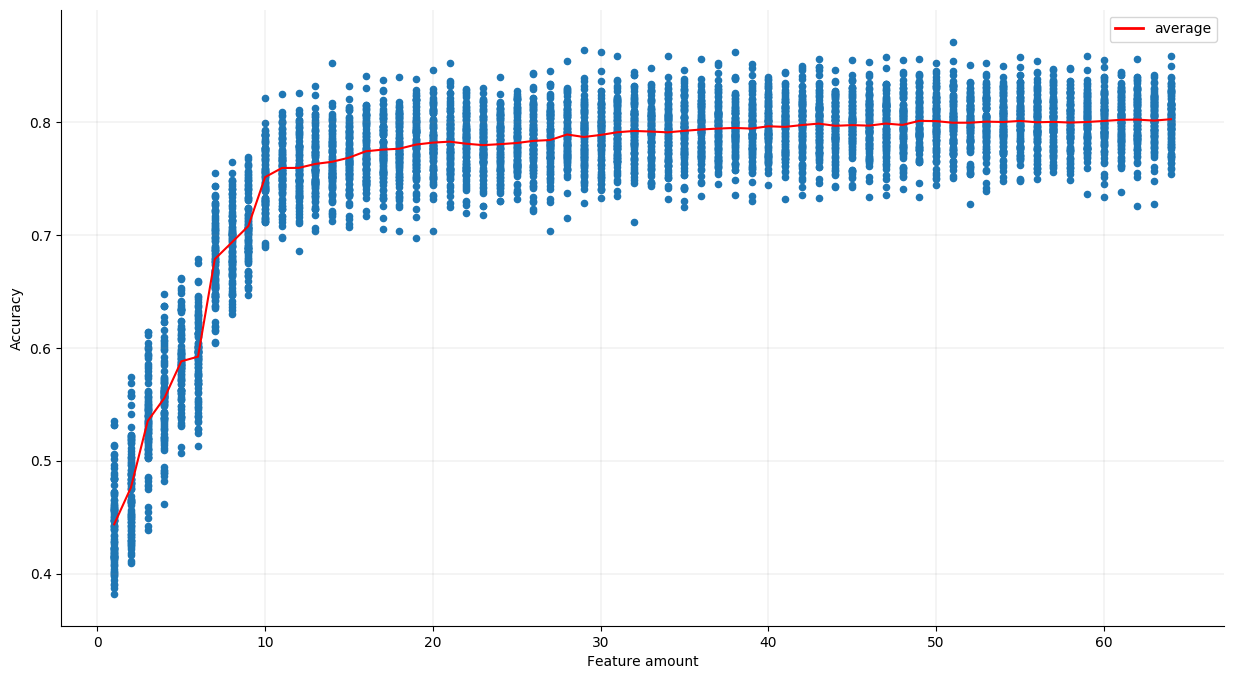
\includegraphics[width=0.8\textwidth]{images/feature_selection.png}
  \caption{\textit{Feature} Auswahl}
  \label{fig:feature_selection}
\end{figure}